\documentclass[12pt]{article}

\usepackage{geometry}
 \geometry{
 a4paper,
 total={170mm,257mm},
 left=20mm,
 right=10mm,
 top=10mm,
 bottom=20mm,
 headheight=75pt
 }
% \usepackage[utf8x]{inputenc}
\usepackage{fontspec}
\setmainfont{Open Sans}
\setsansfont{Noto Sans}
\usepackage{graphicx}
\usepackage{forloop}
\usepackage{subcaption}
\usepackage{url}       % `\url`s
\usepackage{floatrow}
\usepackage{hyperref}
\usepackage{cleveref}
\graphicspath{{resources_quiz_2/}}

\usepackage{fancyhdr}
\pagestyle{fancy}


\renewcommand{\headrulewidth}{0pt}
% \fancyhead[C]{}
% \fancyfoot[]{}


\newcommand\pic[1]{(\cref{#1})} %Где нужно сослаться на рисунок

\hypersetup{
    colorlinks=true,
    linkcolor=blue,
    urlcolor=cyan,
    }

% The preamble ends with the command \begin{document}
\begin{document}
\begin{center}
    \LARGE <<Introduction to Mechanical Engineering>> \\ \textbf{Quiz 2}
\end{center}


\textbf{Task 1}
\begin{enumerate}
    \item Why do we need bearings?
    \item How to fix radial bearing on a shaft. At least 2 possible ways.
\end{enumerate}

\textbf{Task 2}
\begin{enumerate}
    \item Could you name all highlighted parts from the picture \pic{fig:resources_quiz_2/quiz1_task2.png}?
    \item What the difference between bolden and direct extruders.
    \item Could you write the printing process, starting that you have \textit{ideal} CAD model in <<prt>> format.  
\end{enumerate}
\begin{figure}[H]
    \centering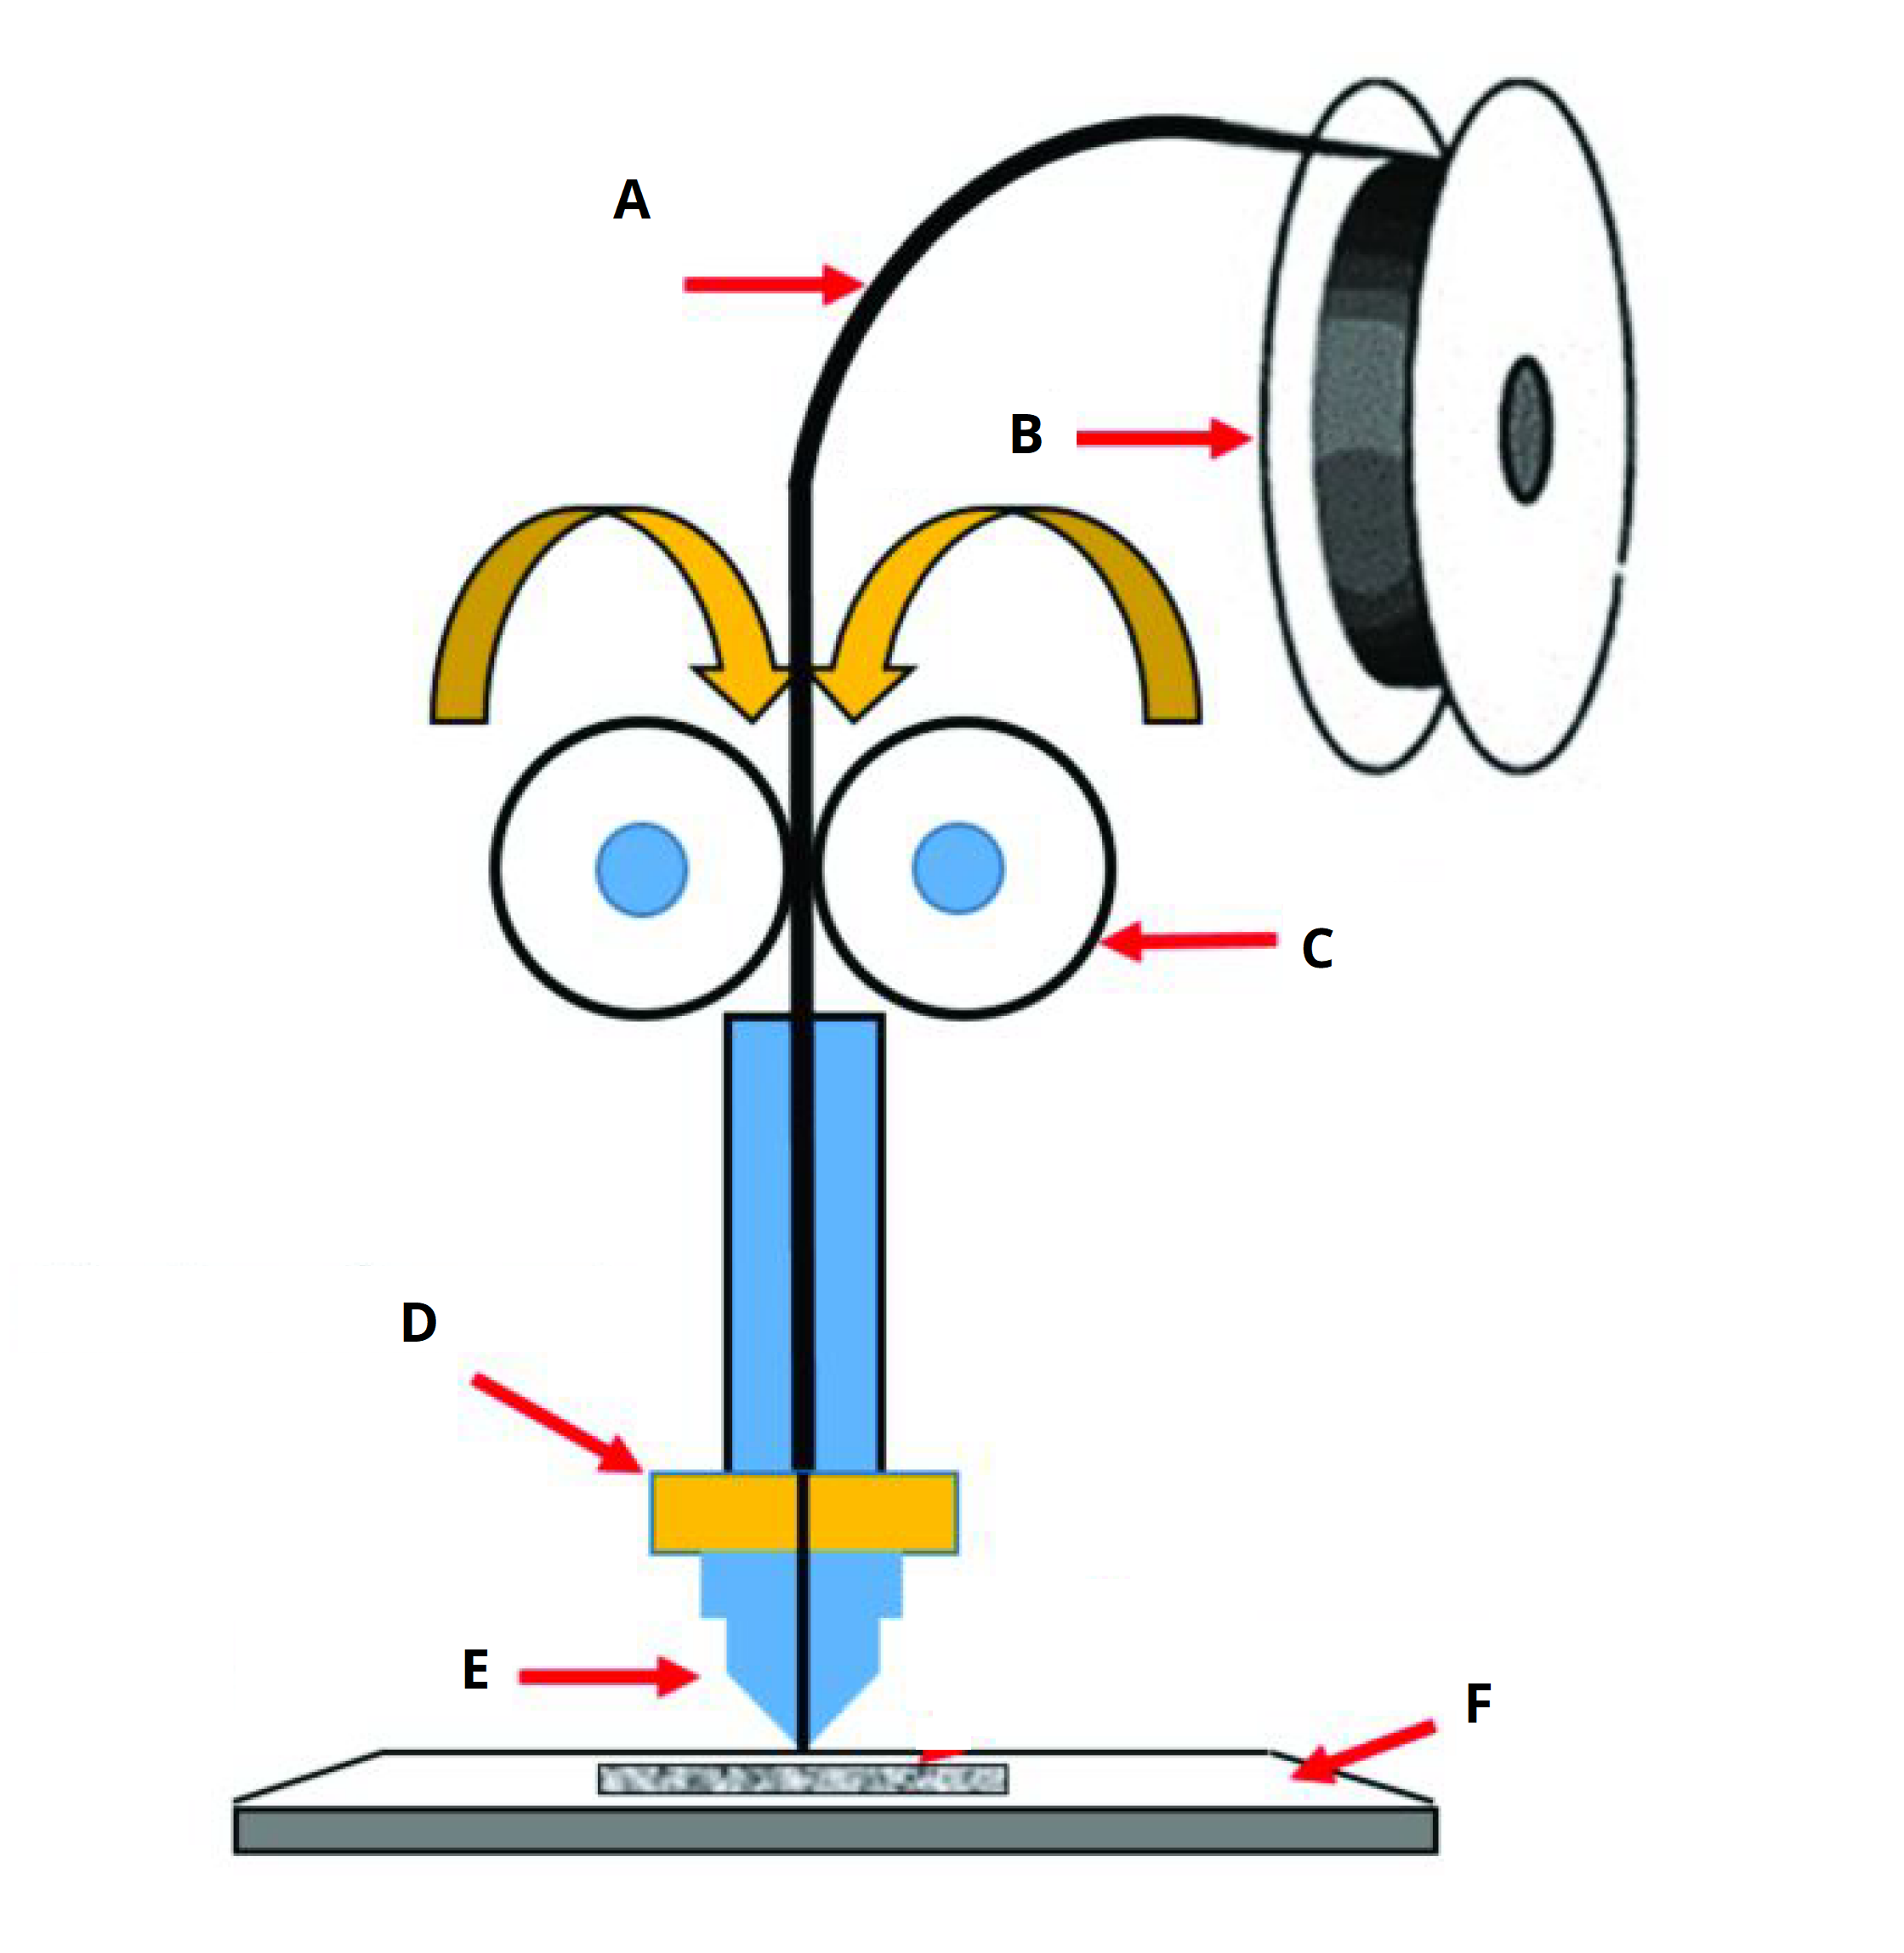
\includegraphics[height=6cm,width=1\textwidth,keepaspectratio]{resources_quiz_2/quiz1_task5.png}
    \caption{Task 2.1}
    \label{fig:resources_quiz_2/quiz1_task2.png}
\end{figure}


\textbf{Task 3}
\begin{enumerate}
    \item Could you name each of type connection on the figure \pic{fig:detach.jpg}. What the benefits of each of them? 
    \item How to connect two shafts together? Why do we need it? 
\end{enumerate}

\begin{figure}[H]
    \centering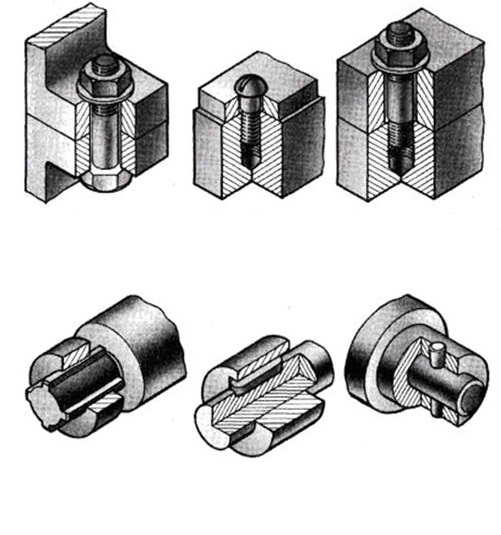
\includegraphics[height=6cm,width=1\textwidth,keepaspectratio]{detach.jpg}
    \caption{Task 3.1}
    \label{fig:detach.jpg}
\end{figure}



\end{document}